
	\documentclass{article}
	\usepackage{amsmath,amssymb}
	\usepackage[inline]{enumitem}
	\usepackage{blindtext}
	\usepackage{booktabs}
	\usepackage{graphicx}
	\usepackage{xcolor}
	\usepackage[vmargin = 1.5in, top = 1in, bottom = 1.2in, letterpaper]{geometry}
	\usepackage{listings}
	\usepackage{courier}
	\usepackage{multicol}
	\usepackage{multirow}
	\usepackage{bm}
	\lstset{
	basicstyle = \small\tt,
	keywordstyle = \tt\color{blue},
	commentstyle = \it\color[cmyk]{1,0,1,0},
	stringstyle = \tt\color[RGB]{128,0,0},
	%frame = single,
	backgroundcolor = \color[RGB]{245,245,244},
	breaklines,
	extendedchars = false,
	xleftmargin = 2em,
	xrightmargin = 2em,
	aboveskip = 1em,
	tabsize = 4,
	showspaces = false
	}
	\begin{document}
	\setcounter{MaxMatrixCols}{20}
	
	% \newfontfamily\courier{Courier New}

	
	\title{STAT 510 Homework 3}
	\author{Yifan Zhu}
	\maketitle
	
	\begin{enumerate}[leftmargin = 0 em, label = \arabic*., font = \bfseries]
	\item 
	\begin{enumerate}
		\item \ 

		\begin{center}
		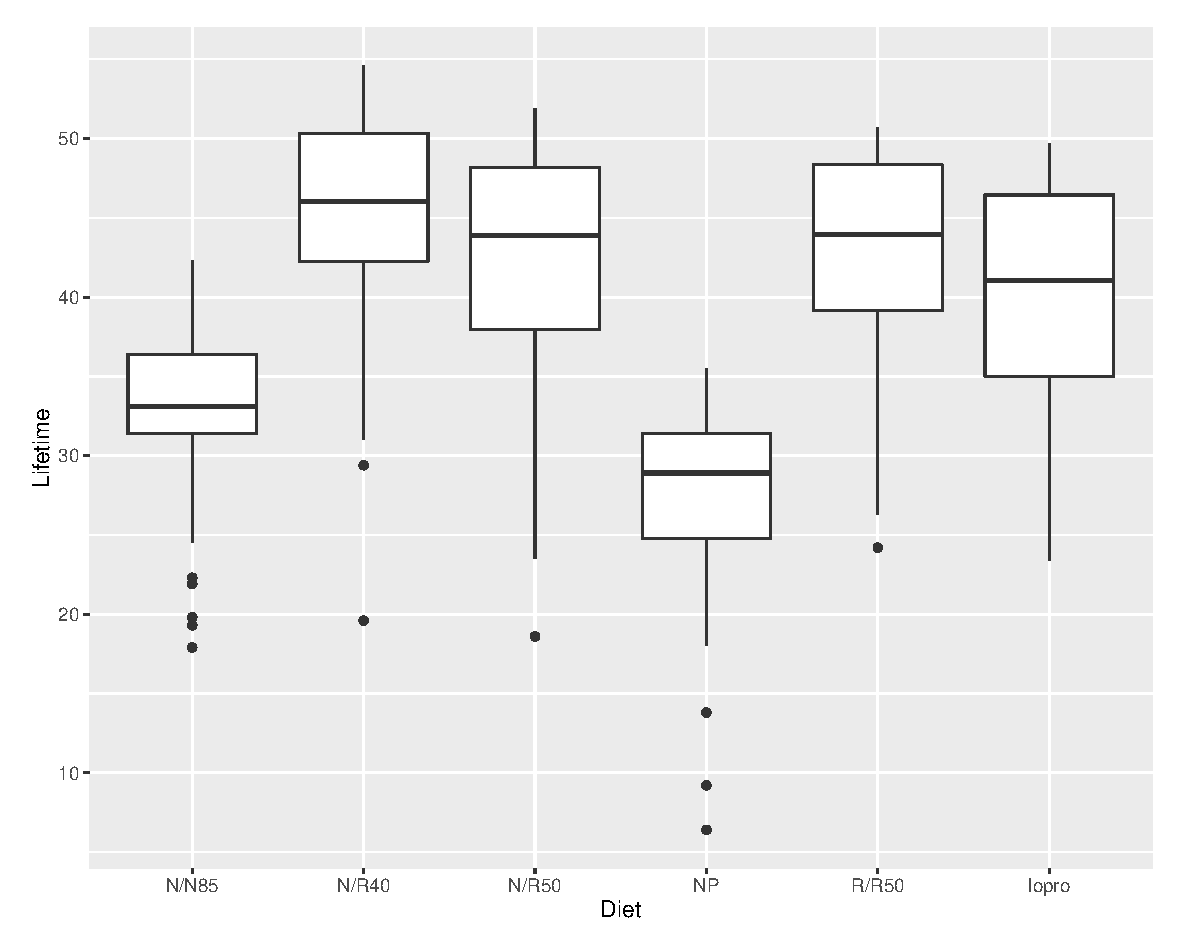
\includegraphics[width = 0.8\textwidth]{boxplot1.eps}
		\end{center}

		\item 
		\[SSE_{full} = 15297\]

		\item 
		\[\hat{\sigma^2} = {\frac{SSE_{full}}{n-r}} = {\frac{15297}{343}} = 44.60\]

		\item 
		\[SSE_{reduced} = 15511\]

		\item 
		\[F = \frac{(SSE_{reduced} - SSE_{full})/(DFE_{reduced} - DFE_{full})}{SSE_{full}/DFE_{full}} = \frac{(15511 - 15297)/1}{15297/343} = 4.8\]

		\item 
		This test is to test the among the mice having these six diet plans,  wheatehr the mice having diet plan N/R50 and N/R50 lopro have the same population life time. 

		\item 
		If the parameter vector $\bm \beta = \begin{bmatrix}
			\beta_1 &\beta_2& \beta_2& \beta_4& \beta_5 &\beta_6
		\end{bmatrix}$ are in the order for N/N85, N/R40, N/R50, NP, R/R50 and N/R50 lopro, then
		\[\bm C = \begin{bmatrix}
			0 & 0 & 1 & 0 & 0 & -1
		\end{bmatrix},\, d = 0\]

		Then
		\[F = \frac{(\bm C \hat{\bm \beta} - d)^T (\bm C (\bm X^T \bm X)^-\bm C^T)^{-1} (\bm C \bm \hat{\bm\beta} - d)/rank(\bm C)}{\hat{\sigma^2}} = 4.8\]
		where $\bm X$ is the model matrix for full model.

		The F statistic is the same as is computed in (e).
	\end{enumerate}

	\item 
	Let $\bm X = \begin{bmatrix}
		1 & 1
	\end{bmatrix}$, then $\bm A = \bm X^T \bm X = \begin{bmatrix}
		1 & 1\\
		1 & 1
	\end{bmatrix}$ is symmetric. Let $\bm G = \begin{bmatrix}
		0 & 0\\
		1 & 0
	\end{bmatrix}$, then
	\[\bm A \bm G \bm A =
	\begin{bmatrix}
		1 & 1\\
		1 & 1
	\end{bmatrix}
	\begin{bmatrix}
		0 & 0\\
		1 & 0
	\end{bmatrix}
	\begin{bmatrix}
		1 & 1\\
		1 & 1
	\end{bmatrix} = \begin{bmatrix}
		1 & 0\\
		1 & 0
	\end{bmatrix}\begin{bmatrix}
		1 & 1\\
		1 & 1
	\end{bmatrix}
	=
	\begin{bmatrix}
		1 & 1\\
		1 & 1
	\end{bmatrix} = \bm A \]

	Thus $\bm G $ is a generalized inverse of the symmetric metrix $\bm A$, but it is not symmetric.

	\item 
	\begin{enumerate}
		\item 
		\begin{align*}
		& rank(\bm X^T \bm X) \leq rank(\bm X)\\
		& rank(\bm X) = rank(\bm P_{\bm X}) = rank(\bm X (\bm X^T \bm X)^- \bm X^T \bm X) \leq rank(\bm X^T \bm X)\\
		\Rightarrow & rank(\bm X) = rank(\bm X^T \bm X)
		\end{align*}


		\item 
		\begin{align*}
		& rank(\bm X) = rank(\bm P_{\bm X} \bm X) \leq rank(\bm P_{\bm X})\\
		& rank(\bm P_{\bm X}) = rank(\bm X (\bm X^T \bm X)^- \bm X) \leq rank(\bm X)\\
		\Rightarrow & rank(\bm X) = rank(\bm P_{\bm X})
		\end{align*}

		\item 
		First we can prove $rank(\bm A \bm P_{\bm X}) = rank(\bm A \bm P_{\bm X})$.
		\begin{align*}
		& rank(\bm A \bm X) = rank(\bm A \bm P_{\bm X} \bm X) \leq rank(\bm A \bm P_{\bm X})\\
		& rank(\bm A \bm P_{\bm X}) = rank(\bm A \bm X (\bm X^T \bm X)^- \bm X^T) \leq rank(\bm A \bm X)\\
		\Rightarrow & rank(\bm A \bm X) = rank(\bm A \bm P_{\bm X})
		\end{align*}
		Then we have 
		\[\bm C (\bm X^T \bm X)^- \bm C^T = \bm A \bm X (\bm X^T \bm X)^- \bm X^T \bm A^T = \bm A \bm P_{\bm X} \bm A^T = \bm A \bm P_{\bm X} \bm P_{\bm X} \bm A^T\]

		Thus $rank(\bm C(\bm X^T \bm X)^- \bm C^T) = rank(\bm A \bm P_{\bm X} (\bm A \bm P_{\bm X})^T) = rank(\bm A \bm P_{\bm X}) = rank(\bm A \bm X) = rank(\bm C) = q$.	

			\item 
			From (c) we know $rank(\bm A \bm X) = rank(\bm A \bm P_{\bm X}) = rank(\bm A)$.	
		
		
	\end{enumerate}
	

	\item 
	\begin{enumerate}
		\item 
		Let the parameter vector in such an order
		\[\begin{bmatrix}
			(S1, F1, 25\%)\\
			(S2, F1, 25\%)\\
			(S1, F2, 25\%)\\
			(S2, F2, 25\%)\\
			(S1, F1, 50\%)\\
			(S2, F1, 50\%)\\
			(S1, F2, 50\%)\\
			(S2, F2, 50\%)\\
			(S1, F1, 75\%)\\
			(S2, F1, 75\%)\\
			(S1, F2, 75\%)\\
			(S2, F2, 75\%)\\
		\end{bmatrix}\]
		Then
		\[\bm C_{(a)} = \begin{bmatrix}
			0&0&0&0&0&0&1&0&0&0&0&0\\

		\end{bmatrix},\, \hat{\mu}_{F2,S1,50\%} = \bm C_{(a)} \hat{\bm \beta} = 233.5\]

		\[se_{(a)} = 11.59\]

		

		\item 
		
		\[\bm C_{(b)} = \begin{bmatrix}
			1/6&1/6&0&0&1/6&1/6&0&0&1/6&1/6&0&0\\
			0&0&1/6&1/6&0&0&1/6&1/6&0&0&1/6&1/6
		\end{bmatrix},\, \begin{bmatrix}
			\hat{\bar{\mu}}_{F1,.,.}\\
			\hat{\bar{\mu}}_{F2,.,.}
		\end{bmatrix} = C_{(b)} \hat{\bm \beta} =\begin{bmatrix}
			214.75\\
			181.08
		\end{bmatrix}\]

		\item 
		\[\bm C_{(c)} = \begin{bmatrix}
			0&1/2&0&1/2&0&0&0&0&0&0&0&0\\

		\end{bmatrix},\, \hat{\bar{\mu}}_{.,S2,25\%} = \bm C_{(c)} \hat{\bm \beta} = 156.25\]

		\item 
		\[se_{(c)} = \sqrt{\hat{\sigma^2} \bm C_{(c)} (\bm X^T \bm X)^- \bm C_{(c)}^T} = 8.20\]

		\item 
		\begin{align*}
		&H_0 : \bar{\mu}_{F1,.,.} = \bar{\mu}_{F2,.,.} (\bm C \bm \beta - d = 0)\\
		&H_a : \bar{\mu}_{F1,.,.} \neq \bar{\mu}_{F2,.,.} (\bm C \bm \beta -d \neq 0)
		\end{align*}
		\begin{align*}
		& \bm C = \begin{bmatrix}
			1/6&1/6&-1/6&-1/6&1/6&1/6&-1/6&-1/6&1/6&1/6&-1/6&-1/6
		\end{bmatrix},\, d = 0\\
		&  F = \frac{(\bm C \hat{\bm \beta} - d)^T (\bm C (\bm X^T \bm X)^-\bm C^T)^{-1} (\bm C \bm \hat{\bm\beta} - d)/rank(\bm C)}{\hat{\sigma^2}} = 25.3\\
		& \textrm{p-value} = 0.0003
		\end{align*}
		Conclusion : Since p-value is small, we decide to reject the null hypothesis and conclude that there is filler type main effect for the fabric loss.

		\item 
		\begin{align*}
		&H_0 : \textrm{there is no three way interaction.} \quad (\bm C \bm \beta - \bm d = 0)\\
		&H_a : \textrm{there is three way interaction.} \quad (\bm C \bm \beta -\bm d \neq 0)
		\end{align*}
		\begin{align*}
		& \bm C = \begin{bmatrix}
			1&-1&-1&1&-1&1&1&-1&0&0&0&0\\
			1&-1&-1&1&0&0&0&0&-1&1&1&-1
		\end{bmatrix},\, \bm d = \begin{bmatrix}
			0\\0
		\end{bmatrix}\\
		&  F = \frac{(\bm C \hat{\bm \beta} - d)^T (\bm C (\bm X^T \bm X)^-\bm C^T)^{-1} (\bm C \bm \hat{\bm\beta} - d)/rank(\bm C)}{\hat{\sigma^2}} = 0.89\\
		& \textrm{p-value} = 0.44
		\end{align*}
		Conclusion : Since p-value is big, we fail to reject the null hypothesis and conclude that there is no three way interaction among the three factors for fabric loss.

		\item 
		\begin{align*}
		&H_0 : \textrm{there is no two way interaction between filler type and filler proportion.} \quad (\bm C \bm \beta - \bm d = 0)\\
		&H_a : \textrm{there is two way interaction between filler type and filler proportion.} \quad (\bm C \bm \beta -\bm d \neq 0)
		\end{align*}
		\begin{align*}
		& \bm C = \begin{bmatrix}
			1/2&1/2&-1/2&-1/2&-1/2&-1/2&1/2&1/2&0&0&0&0\\
			1/2&1/2&-1/2&-1/2&0&0&0&0&-1/2&-1/2&1/2&1/2
		\end{bmatrix},\, \bm d = \begin{bmatrix}
			0\\0
		\end{bmatrix}\\
		&  F = \frac{(\bm C \hat{\bm \beta} - d)^T (\bm C (\bm X^T \bm X)^-\bm C^T)^{-1} (\bm C \bm \hat{\bm\beta} - d)/rank(\bm C)}{\hat{\sigma^2}} = 6.57\\
		& \textrm{p-value} = 0.01
		\end{align*}
		Conclusion : Since p-value is big, we decide to reject the null hypothesis and conclude that there is two way interaction between filler type and filler proportion for fabric loss. 

		
		


	\end{enumerate}
	
	


 	\end{enumerate}


	
	
	
	\end{document}